\chapter{Descrição Detalhada dos Módulos da Suíte Arkos}

\section{Introdução ao Hub de Aplicações}
A arquitetura da Arkos Suite foi projetada sobre um modelo de microsserviços integrados de alta densidade. O ecossistema é composto por plataformas modulares que atuam em simbiose para desatar os gargalos operacionais e escalar a inteligência de negócios.

Garantimos que cada plataforma possua seu próprio motor analítico:

\subsection{Módulo 1: Marketing Intelligence (Inteligência de Mercado)}
O marketing atua como gerador supremo de dados decisórios. Operamos desde o digital analítico até a inteligência profunda, pesquisas quantitativas e qualitativas de mercado, NPS, testes de lançamentos e preços, monitoramento de menções e análise de sentimento nas redes sociais. Tudo convertido em inteligência para a sua tomada de decisão.

\subsection{Módulo 2: Arkos Data (Infraestrutura de Dados)}
Data warehouse, APIs, pipelines e governança de dados. Criamos uma central única que organiza todas as informações da sua empresa, eliminando planilhas soltas e garantido que a diretoria tome decisões baseada em números reais, e não em achismos.

\subsection{Módulo 3: Arkos CRM (Gestão de Relacionamento e Conversão)}
\textbf{Objetivo}: Analisar e escalar a eficiência do funil de conversão comercial da corporação através de ciência de dados.
\begin{itemize}
    \item \textbf{Visão em Tempo Real}: Acompanhamento instantâneo da esteira de leads, interações de atendimento e taxa de fechamento.
    \item \textbf{Cálculo Automatizado de Custos de Vendas (CAC e LTV)}: Permite saber em tempo real o Custo de Aquisição de Cliente (CAC) e o Retorno Financeiro dele ao longo do tempo (LTV). Cruzamos investimentos de captação direto com contratos consolidados, permitindo prever o lucro real por canal de venda.
    \item \textbf{Integração Cross-Sector}: Alerta automático à operação se o fluxo de fechamento demandar aumento imediato de suprimentos no faturamento (ERP) ou contratação de pessoal (Recursos Humanos).
\end{itemize}

\subsection{Módulo 4: Arkos ERP (Gestão de Finanças em Tempo Real)}
\textbf{Objetivo}: Consolidar o motor financeiro e controle operacional em tempo real atrelado a modelagens econométricas preventivas.
\begin{itemize}
    \item \textbf{Fluxo de Caixa Dinâmico}: Toda movimentação, emissão de faturas, contratos vigentes e pedidos de fornecedores são sintetizados instantaneamente para o C-Level.
    \item \textbf{Gestão de Fornecedores e Tickets}: Controle rígido de ordens de compra e fluxos de pagamentos linked a contratos auditáveis, prevenindo vazamentos de capital.
    \item \textbf{Projeções Estatísticas (GPS Financeiro)}: Em vez de registrar o que já foi gasto, o ERP da Arkos faz projeções econométricas alertando se os custos de outros setores superarão as receitas previstas para os próximos 60 dias.
\end{itemize}

\subsection{Módulo 5: Arkos AI Agents (Agentes de IA)}
Agentes autônomos treinados com as regras específicas do seu negócio para resolver chamados e triagens complexas diretamente via canais de atendimento (WhatsApp/Web), reduzindo drasticamente custos de suporte.

\subsection{Módulo 6: Arkos Commerce \& SaaS (Motor de Vendas)}
Motor financeiro robusto 100\% integrado à gestão executiva para e-commerce, recorrência, subscrições de produtos/mensalidades e integrações bancárias diretas automatizadas.

\subsection{Módulo 7: Arkos Growth Agency (Escalabilidade de Marca)}
Squads avançados para empresas parceiras operando desenvolvimento web, landing pages exclusivas, tráfego pago altamente parametrizado e produção audiovisual de marca.

\subsection{Módulo 8: Arkos Strategy Planner (Planejamento Estratégico)}
Formulação e acompanhamento de planejamento estrutural. Oferecemos um sistema autônomo visual que orienta todos os passos, desde a identidade organizacional até a operação tática, ou via consultoria especializada.

\subsection{Módulo 9: Arkos Academy (LMS / EdTech)}
Plataforma de ensino dupla. Internamente, treina e atualiza clientes e líderes em dados e economia competitiva. Externamente, atua como Portal EAD completo para faculdades e escolas, acoplando diagnóstico e predição discente.

\subsection{Módulo 10: Arkos IT \& Infra (Gestão de TI)}
Gestão compartilhada de TI a distância. Atuamos como seu departamento de ponta, elevando a eficiência de empresas com setores legados. Cuidamos da segurança de servidores à administração web.

\subsection{Módulo 11: Arkos Recursos Humanos}
Triagem automatizada de currículos assistida por ferramentas de IA. Executa rankeamento e dossiê de candidatos, gestão de DP (folha de pagamento) e KPIs de capital humano calibrados ao faturamento executivo.

\begin{figure}[H]
  \centering
  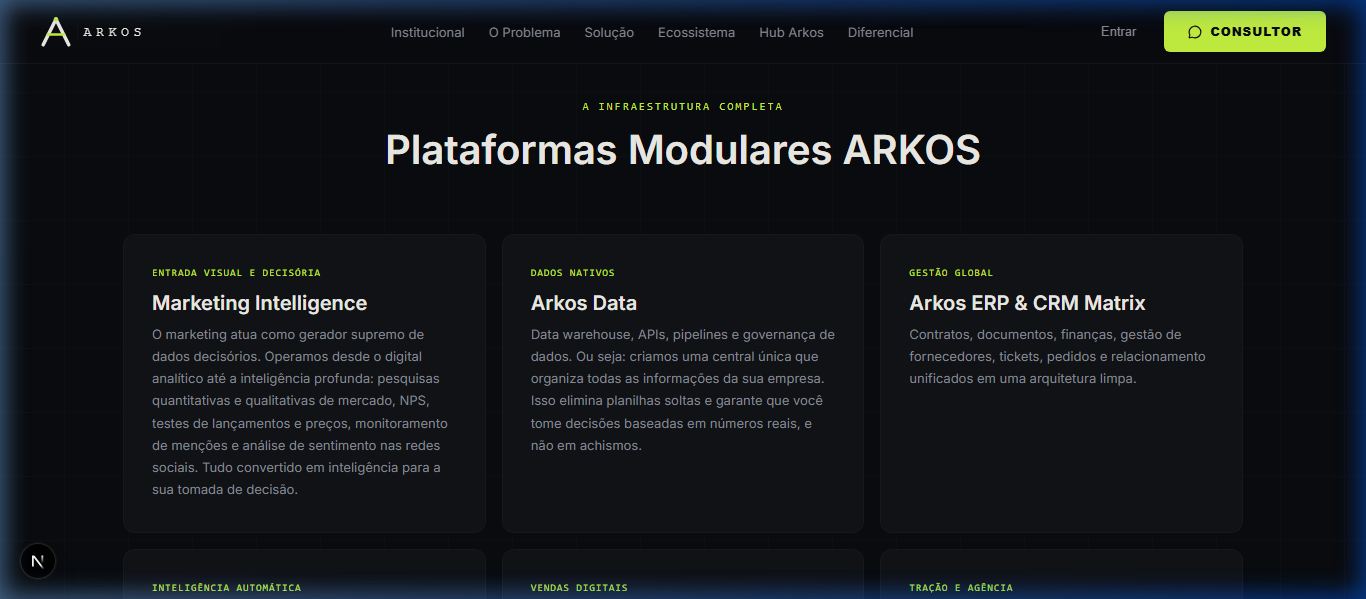
\includegraphics[width=0.85\textwidth]{imagens/hub_modulos_lista.png}
  \caption{Visão expandida da Suite Arkos: 11 Plataformas modulares desenhadas para agir em simbiose operacional contínua.}
\end{figure}

\section{Nossos Diferenciais Competitivos}
A Arkos não compete com softwares isolados (SaaS de Prateleira). Nossa proposta diferencia-se por entregar \textbf{Infraestrutura e Inteligência Ativa}:
\begin{itemize}
    \item \textbf{Operação Analítica de Alto Nível}: Cruzamento de dados cross-módulos com validação em tempo real. Menos de 5\% das empresas conseguem esse nível de assertividade econométrica sem terceirizar BIs manuais.
    \item \textbf{Letramento Nativo de Equipe}: Os algoritmos preditivos e dashboards são construídos para dar \textbf{autonomia decisória} à corporação parceira de forma independente.
    \item \textbf{Arquitetura em 4 Camadas}: Processamento seguro desde a ingestão passiva de Fontes Isoladas (ERP, planilhas), passando pelo \textbf{Data Lake Node} (ETL), Processamento de Predictive Analytics até a ponta da interface rodando inteligência natural.
\end{itemize}

\begin{figure}[H]
  \centering
  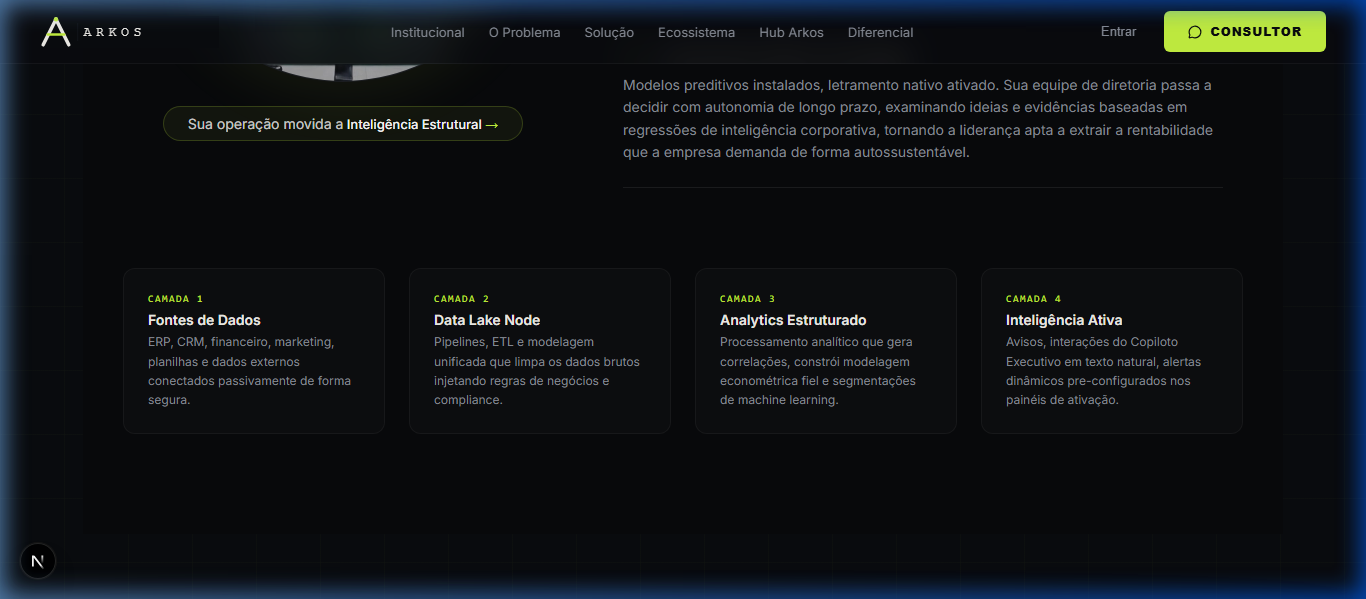
\includegraphics[width=0.85\textwidth]{imagens/diferenciais.png}
  \caption{Mesa operacional da @ARKOS: Operação Analítica de Alto Nível de Infraestrutura.}
\end{figure}

\section{Ferramentas de Suporte Nativas (.Micro-Apps)}
Além das plataformas matriciais de gestão, a Workspace da Arkos fornece em sua malha interna aplicativos focados em produtividade e colaboração unificada:
\begin{itemize}
    \item \textbf{Arkos Cloud}: Buffer seguro para classificar e auditar mídias e entregáveis documentais.
    \item \textbf{Arkos Rooms}: Reuniões remotas com transcrição IA e auto-geração de Atas em PDF direto para o financeiro ou CLM.
    \item \textbf{Arkos Flow}: Painéis Scrum e Kanban nativos para gestão ágil de projetos por setor em tempo real.
    \item \textbf{Arkos Connect}: Feed corporativo interno para rituais e avisos com total confidencialidade.
    \item \textbf{Arkos LiveTranslate & SmartBooking}: Agendamentos vinculados a disparos de WhatsApp e pontes de tradução para ligações globais.
\end{itemize}

\begin{figure}[H]
  \centering
  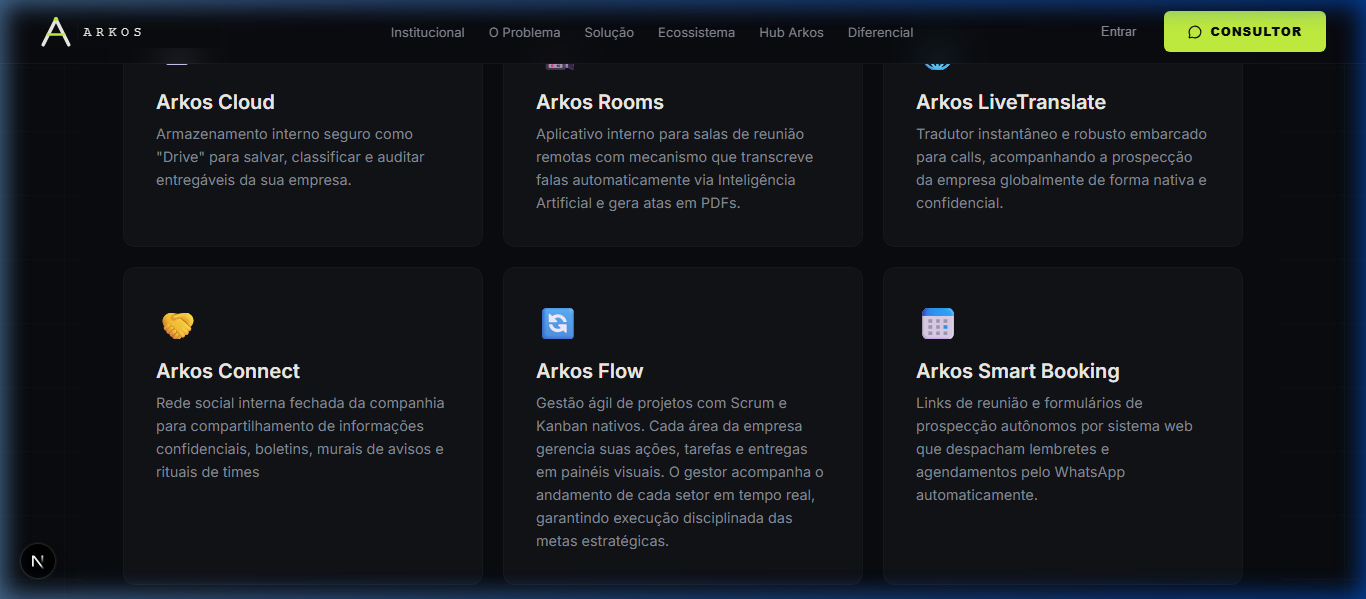
\includegraphics[width=0.85\textwidth]{imagens/micro_apps_grid.png}
  \caption{Hub de Aplicações de Micro-Apps nativos prontas para a rotina executiva.}
\end{figure}

\pagebreak
